\section{Architecture Integration}

\subsection{Model Support}

\begin{table}[H]
\centering
\small
\begin{tabular}{lllll}
\toprule
\textbf{Model} & \textbf{Attention class} & \textbf{Nested?} & \textbf{RoPE?} & \textbf{GQA?} \\
\midrule
DistilBERT & \texttt{MultiHeadSelfAttention} & No & No & No \\
RoBERTa & \texttt{BertSelfAttention} (nested) & Yes & No & No \\
GPT-2 & \texttt{GPT2Attention} (Conv1D) & No & No & No \\
Qwen3.5 & \texttt{Qwen3Attention} & No & Yes & Yes \\
\bottomrule
\end{tabular}
\end{table}

\subsection{Weight Extraction}

Res-SVD uses the same weight extraction as companion modules:

\subsubsection{DistilBERT}

\begin{lstlisting}
extracted["q"] = src.q\_lin.weight
extracted["k"] = src.k\_lin.weight
extracted["v"] = src.v\_lin.weight
extracted["o"] = src.out\_lin.weight
\end{lstlisting}

\subsubsection{RoBERTa (nested)}

\begin{lstlisting}
s = src.self
extracted["q"] = s.query.weight
extracted["k"] = s.key.weight
extracted["v"] = s.value.weight
extracted["o"] = src.output.dense.weight
\end{lstlisting}

\subsubsection{GPT-2 (Conv1D)}

\begin{lstlisting}
w = src.c\_attn.weight.t()
q\_w, k\_w, v\_w = w.chunk(3, dim=0)
\end{lstlisting}

\subsubsection{Qwen}

Direct extraction from named projections.

\subsection{Nested Encoder Handling}

For RoBERTa/BERT, the output projection is applied externally. 
Res-SVD handles this via \textbf{identity initialization} of the output projection:

\begin{lstlisting}
if proj\_key == "o" and self.is\_nested\_encoder:
    temp\_linear = nn.Linear(target.in\_features, target.out\_features)
    nn.init.eye\_(temp\_linear.weight)
    nn.init.zeros\_(temp\_linear.bias)
    new\_layer = ResSVDLinear.from\_linear(temp\_linear, ...)
    target.load\_state\_dict(new\_layer.state\_dict())
\end{lstlisting}

Then in forward:
\begin{lstlisting}
if self.is\_nested\_encoder:
    return context  # skip out\_proj
\end{lstlisting}

\subsection{The `ResSVDLinear` Module}

Located in \texttt{framework/compression\_engine/res\_svd.py}. Structure:

\begin{lstlisting}
class ResSVDLinear(nn.Module):
    def \_\_init\_\_(self, in\_features, out\_features, base\_rank, residual\_rank,
                 scaling=1.0, factorize\_base=True, bias=True):
        super().\_\_init\_\_()
        self.V\_base = nn.Parameter(torch.empty(base\_rank, in\_features))
        self.U\_base = nn.Parameter(torch.empty(out\_features, base\_rank))
        self.lora\_A = nn.Parameter(torch.empty(residual\_rank, in\_features))
        self.lora\_B = nn.Parameter(torch.empty(out\_features, residual\_rank))
        if bias:
            self.bias = nn.Parameter(torch.empty(out\_features))
        self.scaling = scaling
    
    @classmethod
    def from\_linear(cls, linear, base\_rank, residual\_rank, ...):
        W = linear.weight.data.float()
        U, S, Vt = torch.linalg.svd(W, full\_matrices=False)
        
        # Base
        U\_b = U[:, :base\_rank]
        S\_b = S[:base\_rank]
        Vt\_b = Vt[:base\_rank, :]
        
        # Residual
        W\_b = (U\_b * S\_b) @ Vt\_b
        R = W - W\_b
        U\_r, S\_r, Vt\_r = torch.linalg.svd(R, full\_matrices=False)
        
        # LoRA init
        S\_r\_sqrt = torch.sqrt(S\_r[:residual\_rank])
        B\_init = U\_r[:, :residual\_rank] * S\_r\_sqrt
        A\_init = S\_r\_sqrt[:, None] * Vt\_r[:residual\_rank, :]
        
        layer = cls(...)
        layer.U\_base.data = U\_b
        layer.V\_base.data = Vt\_b
        layer.lora\_B.data = B\_init
        layer.lora\_A.data = A\_init
        return layer
    
    def forward(self, x):
        h\_b = F.linear(x, self.V\_base)
        y\_b = F.linear(h\_b, self.U\_base)
        h\_r = F.linear(x, self.lora\_A)
        y\_r = F.linear(h\_r, self.lora\_B)
        return y\_b + self.scaling * y\_r + self.bias
\end{lstlisting}

\subsection{Freezing Base Weights}

\begin{lstlisting}
self.U\_base.requires\_grad = False
self.V\_base.requires\_grad = False
# lora\_A, lora\_B remain trainable
\end{lstlisting}

\subsection{Injection}

The \texttt{inject\_res\_svd} hook:
\begin{itemize}
\item Handles whole-model traversal
\item Finds attention modules
\item Creates new \texttt{ResSVDAttention} with weight transfer
\item \textbf{Returns \texttt{None} on failure} (silent fallback)

\end{itemize}
\begin{lstlisting}
except Exception as e:
    logger.error("inject\_res\_svd failed at layer \%d: \%s", layer\_idx, e)
    return None
\end{lstlisting}

\subsection{Failure Modes}

\begin{table}[H]
\centering
\small
\begin{tabular}{ll}
\toprule
\textbf{Failure} & \textbf{Response} \\
\midrule
Missing projection & \texttt{copy\_weights} raises RuntimeError \\
Small Frobenius norm & Raises RuntimeError \\
Injection error & Returns None (silent) \\
\bottomrule
\end{tabular}
\end{table}

\subsection{Registry}

\begin{lstlisting}
@ATTENTION\_REGISTRY.register("res\_svd")
@ATTENTION\_REGISTRY.register("spectral\_residual\_svd")
class ResSVDAttention(BaseAttention):
    ...
\end{lstlisting}

\subsection{Cross-Attention}

\begin{lstlisting}
if encoder\_hidden\_states is not None:
    raise NotImplementedError(...)
\end{lstlisting}
\begin{lstlisting}

---
\end{lstlisting}

\begin{figure}[H]
\centering
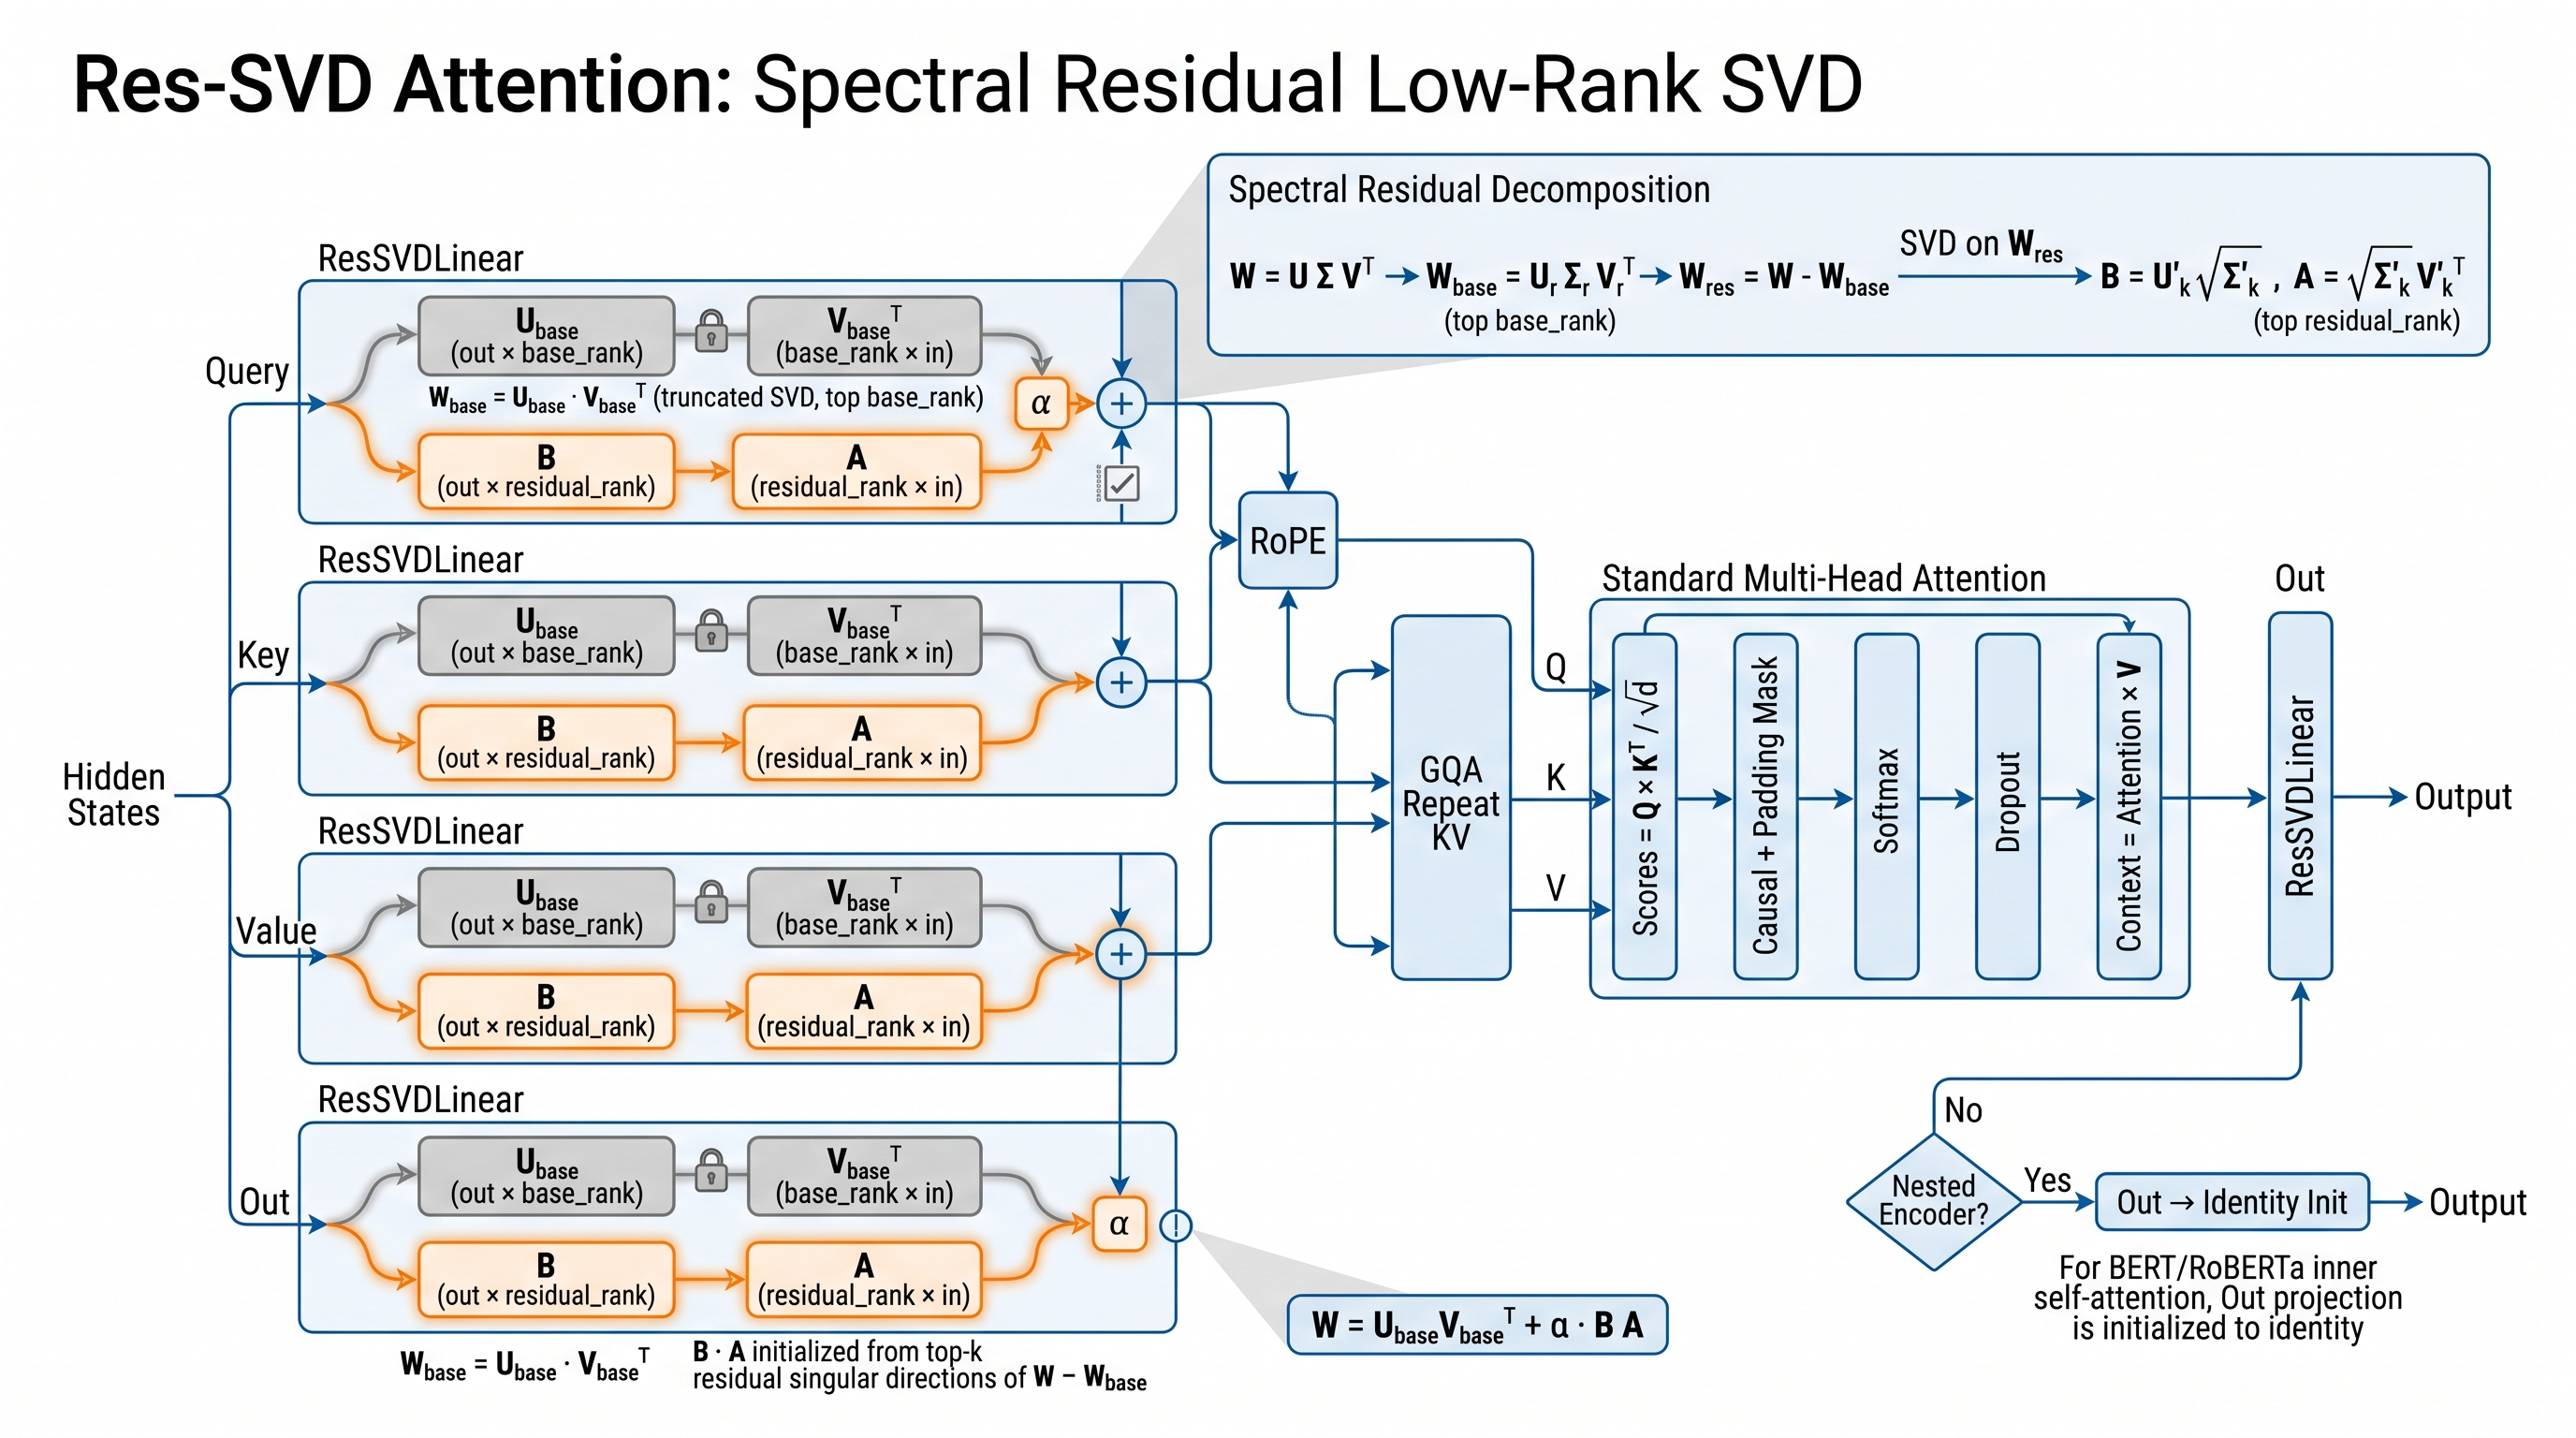
\includegraphics[width=\linewidth]{figures/architecture.jpeg}
\caption{High-level architectural diagram of res\_svd.}
\label{fig:arch\_res-svd}
\end{figure}

